% INSTRUCTIONS:
% To compile this file, run "latex HW_example";  you need to do it TWICE
%    to get the cross-references (to equations, etc) to show correctly.
% Figures can be included as shown below.  If you don't have a figure,
%    comment out those lines using % signs at the beginning of each line,
%    or else just keep hitting RETURN when LaTeX gives an error message
%    saying that it can't find the figure file.
% Run "dvips HW_example.dvi" to make a Postscript file HW_example.ps,
%    and then "ps2pdf HW_example.ps" to make a PDF file HW_example.pdf.

\documentclass[12pt]{article}
\usepackage{graphicx,indentfirst}

\pagestyle{plain}
\baselineskip 18pt
\textwidth 6.5in
\textheight 7.8in
\oddsidemargin 0.1in
\evensidemargin 0.1in
\topmargin 0.3in

\newcommand{\be}{\begin{equation}}
\newcommand{\ee}{\end{equation}}
\newcommand{\reff}[1]{(\ref{#1})}


\begin{document}

\title{Computational Physics \\ Homework 4}
\author{Yi-Hsuan Hsu}
\date{10/16/2014}
\maketitle

\section{Problem 1}
Newtonian mechanic describes planetary orbit in second order differential equation.    
\begin{equation}
		\frac{d^2u}{d\phi^2}+u=\frac{GM}{l^2}\\
\end{equation}
Solving the equation analytically and numerically. Euler method, two stages Runge-Kutta and four stages Runge-Kutta method are applied. Compare behaviors such as error, convergence rate between each method.


\subsection{Theory}
$(a)$prove exact solution of equation (1) is
\begin{eqnarray}
u=\frac{GM}{l^2}(1+\epsilon cos\phi)
\end{eqnarray}
Explicitly, we have homogenious and inhomogenious solution 

\begin{eqnarray}
	u_{0}&=&\frac{GM}{l^2}\\
	u_{H}&=&Acos(\phi+\phi_0)
\end{eqnarray}
where $A$ and $\phi_0$ are arbitrary parameter depends on initial condition. We choose $\phi_0=0$, and $A=\epsilon\frac{GM}{l^2}$where
\begin{equation}
	\epsilon=\sqrt{1+2EL^2/(GMm)^2}
\end{equation}
hence, the exact solution is $u_H$ plus $u_0$

\begin{eqnarray}
	u(\phi)&=&u_0+u_H\nonumber\\
		&=&\frac{GM}{l^2}(1+\epsilon cos(\phi))	
\end{eqnarray}
An ellipse with eccentricity $\epsilon$ are obtained.

\subsection{Algorithms}
\subsubsection{Euler Method}
Suppose we we want to solve a first order ODE with initial value
\begin{equation}
	y'(t)=f(t,y(t)),  y(t_0)=y_0 \nonumber
\end{equation}
Set step size$h$, one step of Euler method from $t_n$ to $t_{n+1}$ is
\begin{equation}
	y_{n+1}=y_n+hf(t_n,y_n)
\end{equation}
Now derive local truncation error, using Taylor expansion in equation (8),
\begin{equation}
	y(t_{n+1}+h)=y(t_n)+hy'(t_n)+\frac{1}{2}y''(t_n)+O(h^3)
\end{equation}
Therefore, 
\begin{equation}
	\delta=y(t_0+h)-y_1=\frac{1}{2}h^2y''(t_0)+O(h^3)
\end{equation}
which shows that truncation error is proportional to $h^2$.

In this homework, we can reduce second order ODE into two first order ODE problem.
\begin{eqnarray}
	\frac{du}{d\phi}=v=f_1(u,n,t)&&,u(0)=1+\epsilon,u'(0)=0\nonumber\\
	\frac{dv}{d\phi}=-u+1=f_2(v,n,t)&&,v(0)=0,v'(0)=0
\end{eqnarray}
where we let $\frac{GM}{l^2}=1$ with proper unit. Therefore, Euler method become
\begin{eqnarray}
	u_{n+1}=u_n+h f_1(u_n,v_n,t_n)\nonumber\\
	v_{n+1}=v_n+h f_2(u_n,v_n,t_n)
\end{eqnarray}



\subsubsection{2-order Runge-Kutta Method}
2-order Runge-Kutta method are given by formula
\begin{equation}
	y_{n+1}=y_n+hf(t_n+\frac{h}{2}),y_n+\frac{h}{2}f(t_n,y_n)
\end{equation}
truncation error is proportional to $h^2$.

In our practice, the formula become
\begin{eqnarray}
	&&l_1=f_1(u_n+\frac{h}{2}f_1(u_n,v_n,t_n),v_n,t_n+\frac{h}{2})\nonumber\\
	&&k_1=f_2(u_n+\frac{h}{2}f_1(u_n,v_n,t_n),v_n+\frac{h}{2}f_2(u_n,v_n,t_n),t_n+\frac{h}{2})\nonumber\\
	&&u_{n+1}=u_n+h l_1\nonumber\\
	&&v_{n+1}=v_n+h k_1
\end{eqnarray}

\subsubsection{4-order Runge-Kutta Method}
4-order Runge-Kutta method are given by formula
\begin{eqnarray}
	&&y_{n+1}=y_n+\frac{h}{6}(k_1+ 2k_2+2k_3+k4)\nonumber\\
	&&k_1=f(t_n,y_n)\nonumber\\
	&&k_2=f(t_n+\frac{h}{2},y_n+\frac{h}{2}k_1)\nonumber\\
	&&k_3=f(t_n+\frac{h}{2},y_n+\frac{h}{2}k_2)\nonumber\\
	&&k_4=f(t_n+h,y_n+hk_3)
\end{eqnarray}
truncation error is proportional to $h^4$.

Again, in our problem the formula become
\begin{eqnarray}
	&&l_1=f_1(t_n,u_n,v_n)\nonumber\\
	&&k_1=f(t_n,u_n+\frac{h}{2}l_1,v_n)\nonumber\\
	&&l_2=f(t_n+\frac{h}{2},u_n+\frac{h}{2}l_1,v_n+\frac{h}{2}k_1)\nonumber\\
	&&k_2=f(t_n+\frac{h}{2},u_n+\frac{h}{2}l_2,v_n+\frac{h}{2}k_1)\nonumber\\
	&&l_3=f(t_n+\frac{h}{2},u_n+\frac{h}{2}l_2,v_n+\frac{h}{2}k_2)\nonumber\\
	&&k_3=f(t_n+\frac{h}{2},u_n+\frac{h}{2}l_3,v_n+\frac{h}{2}k_2)\nonumber\\
	&&l_4=f(t_n+h,u_n+hl_3,v_n+2k_3)\nonumber\\
	&&k_4=f(t_n+h,u_n+hl_4,v_n+2k_3)\nonumber\\
	&&u_{n+1}=u_n+\frac{h}{6}(l_1+ 2l_2+2l_3+l4)\nonumber\\
	&&v_{n+1}=v_n+\frac{h}{6}(k_1+ 2k_2+2k_3+k4)
\end{eqnarray}
\subsection{Sample output}
\begin{figure}[h!]
	\begin{center}
		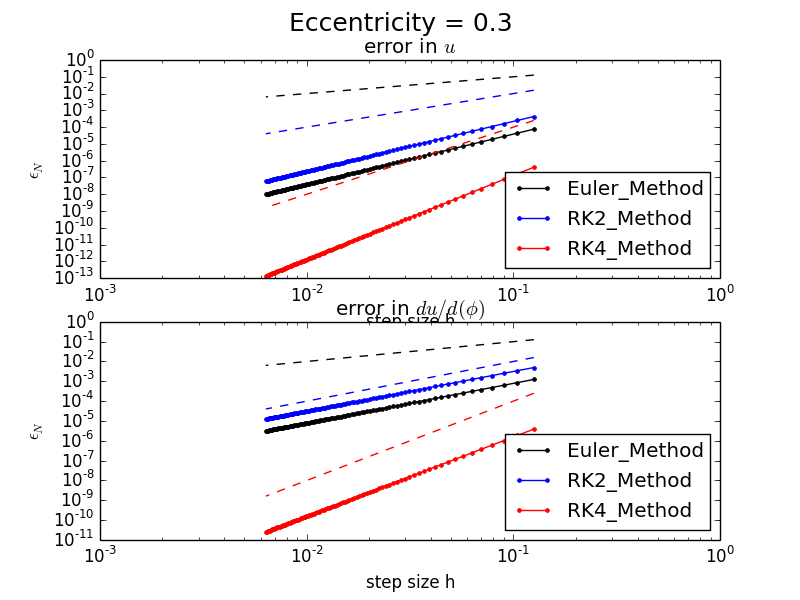
\includegraphics[width=0.8\textwidth]{error_ecc03.png}
		\caption{Sample output eccentricity=0.3}
		\label{fig1}
	\end{center}
\end{figure}
\begin{figure}[h!]
	\begin{center}
		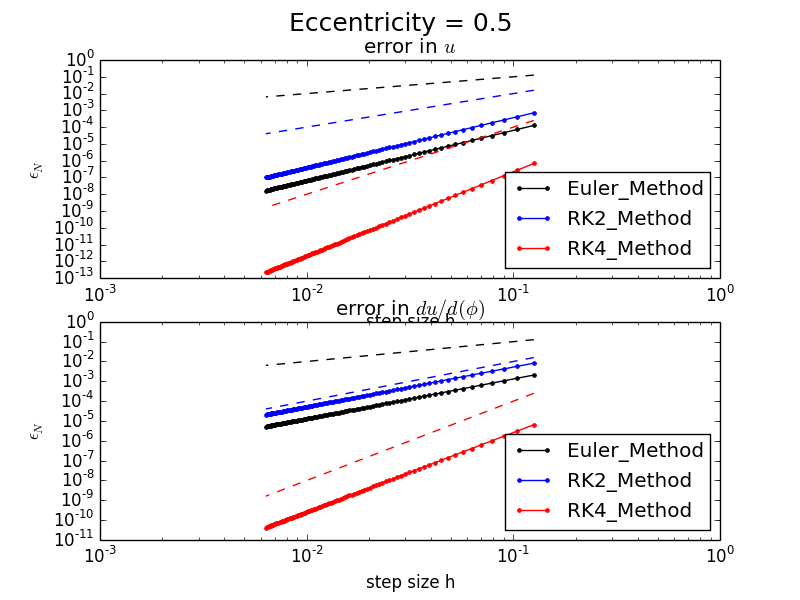
\includegraphics[width=0.8\textwidth]{error_ecc05.png}
		\caption{Sample output eccentricity=0.5}
		\label{fig2}
	\end{center}
\end{figure}
\begin{figure}[h!]
	\begin{center}
		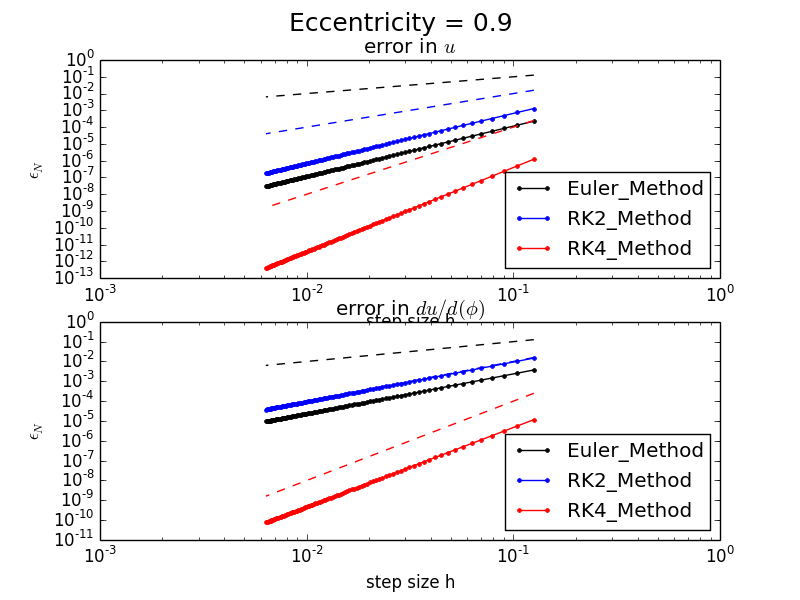
\includegraphics[width=0.8\textwidth]{error_ecc09.png}
		\caption{Sample output eccentricity=0.9}
		\label{fig3}
	\end{center}
\end{figure}
From sample output, RK2 and RK4 converge roughly follow the theoritical predict. But, Euler method go faster then it should be.


\section{Problem 2} 
\subsection{Theory}
General relativity corrects equation (1) to 
\begin{equation}
	\frac{d^2u}{d\phi^2}+u=\frac{GM}{l^2}+\frac{3GM}{c^2}u^2
\end{equation}
or rewrite into
\begin{equation}
	u''+u=1+3\lambda u^2
\end{equation}
from perturbation theory, we assume the solution is homogenious exact solution plus perturbation term
\begin{equation}
	u=u_0+\lambda*f_1(\phi)
\end{equation}
where $u_0=1+\epsilon cos(\phi)$ as we shown before, and $\lambda$ is a small number. Substitute equation(19) into equation (18), we have
\begin{eqnarray}
	\lambda f''+\lambda f &&= 3 \lambda(1+\epsilon cos(\phi))^2\nonumber\\
	f''+f &&=3(1+2\epsilon cos(\phi))+O(\epsilon^2)
\end{eqnarray}
Solving $f(\phi)$, we have
\begin{equation}
	f(\phi)=3(1+\epsilon \phi sin(\phi))
\end{equation}
Therefore, equation (19) becomes
\begin{eqnarray}
	u=1+\epsilon cos(\phi)+3\lambda(1+\epsilon \phi sin(\phi))
\end{eqnarray}
for small $\lambda$, one can write
\begin{eqnarray}
	cos(\phi(1-3\alpha))&&=cos\phi cos3\lambda\phi+sin\phi sin3\lambda\phi\nonumber\\
	&&\approx cos\phi+3\lambda\phi sin\phi\\
	u&&\approx 1+\epsilon cos[\phi(1-3\lambda)]
\end{eqnarray}
finally,
\begin{equation}
	\Delta\phi^{shift}=\frac{2\pi}{1-3\lambda}-2\pi=6\pi\lambda+O(\lambda^2)
\end{equation}
shows that $\Delta\phi^{shift}$ is proportional to small number of $\lambda$, the slope is $6\pi$.

\subsection{Algorithm}
4-order Runge-Kutta Method were described before. Here we just modified $f_2(u,v,t)$ into
\begin{equation}
	\frac{dv}{d\phi}=f_2(u,v,t)=-u+1+3\lambda u^2
\end{equation}

\subsection{Sample output}
\begin{figure}[h!]
	\begin{center}
		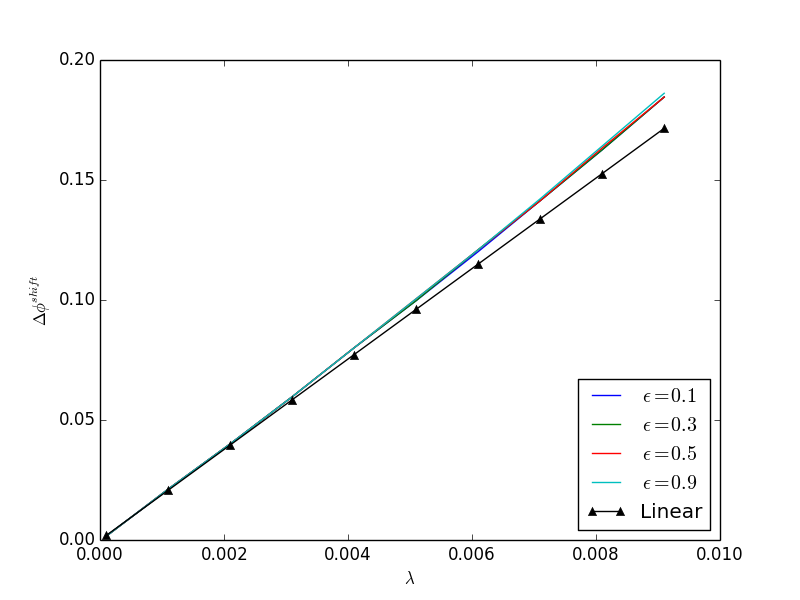
\includegraphics[width=0.8\textwidth]{problem2a.png}
		\caption{Relationship between $\lambda$ and $\Delta\phi^{shift}$ follow linear approximation when $\lambda$ is small. When $\lambda$ goes larger, the numerical approach behave like quadratic due to higher order term}
		\label{fig4}
	\end{center}
\end{figure}

\subsection{problem 2 (c)}
From NASA database, the key fact of Mercury 
\begin{eqnarray}
	G&&=6.67\times 10^{11} m^3 kg^{-1} s^{-2}\nonumber\\
	M_{sun}&&=1.988\times 10^{30} kg\nonumber\\
	c&&=3.0\times 10^8 ms^{-1}\nonumber\\
	R_{orbit}&&=46\times 10^9 m\nonumber\\
	v&&=58.98\times 10^3 ms^{-1}\nonumber\\
	T_{period}&&=87.968 days
\end{eqnarray}
Hence
\begin{equation}
	\lambda=\frac{GM}{lc}^2=2.6541\times10^{-8}
\end{equation}
Therefore, $\Delta\phi^{shift} per period$
\begin{equation}
	\Delta\phi^{shift}=6\pi\lambda=0.103191"
\end{equation}
and shift per century are given by
\begin{equation}
	\Delta\phi^{shift}_{century}=\Delta\phi^{shift}\frac{100}{T_{period}}=42.8458"
\end{equation}


\end{document}

\begin{figure}[h!]
	\begin{center}
		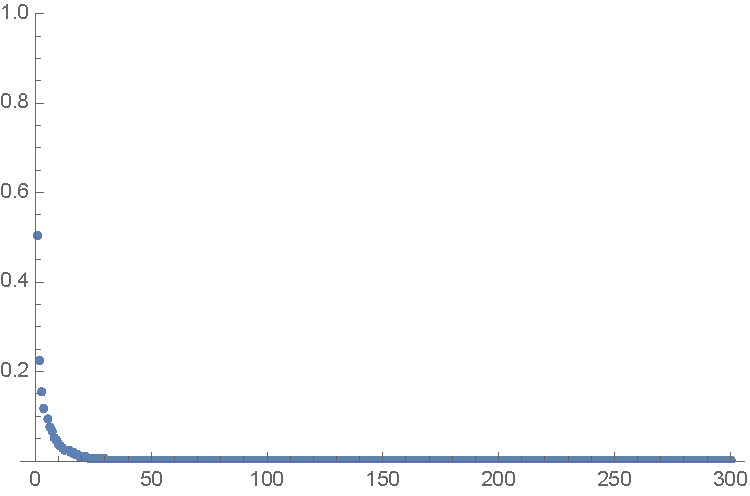
\includegraphics[width=0.4\textwidth]{a_09.pdf}
		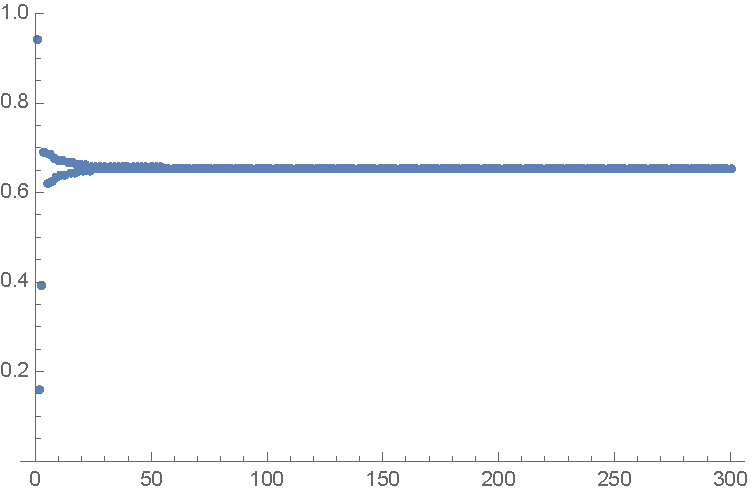
\includegraphics[width=0.4\textwidth]{a_29.pdf}
		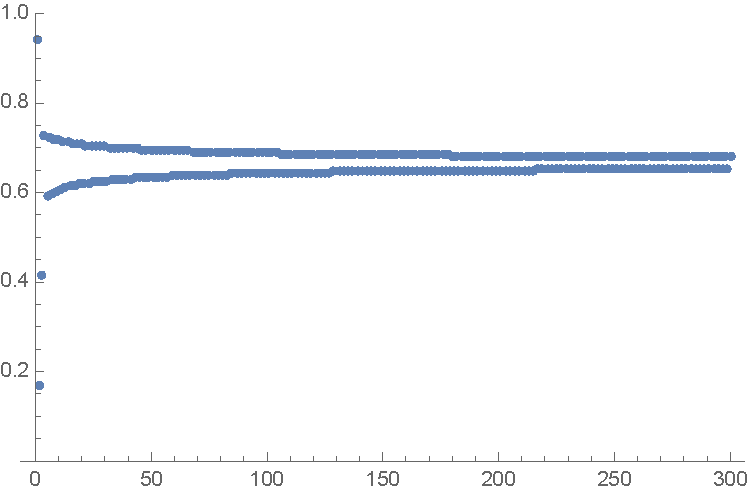
\includegraphics[width=0.4\textwidth]{a_30.pdf}
		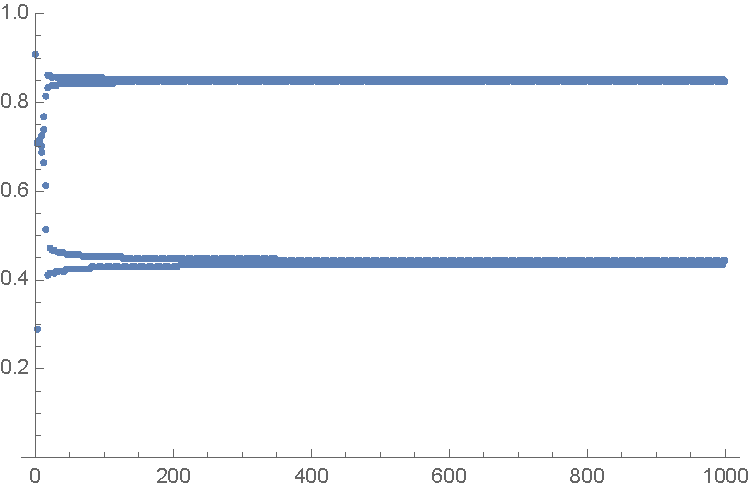
\includegraphics[width=0.4\textwidth]{a_3449.pdf}
		\caption{logistic map. Upper, left a=0.99, right a=2.9. Lower, left a=3.0, right a=3.4494.}
	\end{center}
\end{figure}

\begin{figure}[b!]
	\begin{center}
		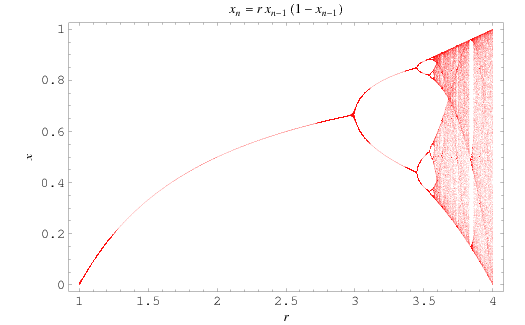
\includegraphics[width=0.8\textwidth]{logistic_map.png}
		\caption{bifurcation diagram of the logistic map. Pic. from Mahtworld}
		\label{fig1}
	\end{center}
\end{figure}


\begin{table}[h!]
	\begin{tabular}{c|lr}
		\hline
		A & $Table$ & Is\\ 
		Messy & To & Write\\
		\hline
	\end{tabular}
\end{table}


\begin{table}[h]
	\begin{center}
		\begin{tabular}{c|c}
			\hline
			period & bifurcation point a\\ 
			\hline
			2 & $0.7199616841972$ \\
			4 & $0.8332663532346$\\
			8 & $0.8591690091416$\\
			16& $0.8640801075000$*\\
			\hline
		\end{tabular}
	\end{center}
	\caption{Numerical approach to recursion sin function. First three are searching by bisection method, $\epsilon<10^{-10}$. *Last one is using step-in method, accuracy$\epsilon<10^{-5}$, although steps are much smaller than that.}
\end{table}
